%; whizzy chapter
% -initex iniptex -latex platex -format platex -bibtex jbibtex -fmt fmt
% 以上 whizzytex を使用する場合の設定。

%     Tokyo Debian Meeting resources
%     Copyright (C) 2011 Junichi Uekawa
%     Copyright (C) 2011 Nobuhiro Iwamatsu

%     This program is free software; you can redistribute it and/or modify
%     it under the terms of the GNU General Public License as published by
%     the Free Software Foundation; either version 2 of the License, or
%     (at your option) any later version.

%     This program is distributed in the hope that it will be useful,
%     but WITHOUT ANY WARRANTY; without even the implied warranty of
%     MERCHANTABILITY or FITNESS FOR A PARTICULAR PURPOSE.  See the
%     GNU General Public License for more details.

%     You should have received a copy of the GNU General Public License
%     along with this program; if not, write to the Free Software
%     Foundation, Inc., 51 Franklin St, Fifth Floor, Boston, MA  02110-1301 USA

%  preview (shell-command (concat "evince " (replace-regexp-in-string "tex$" "pdf"(buffer-file-name)) "&"))
% 画像ファイルを処理するためにはebbを利用してboundingboxを作成。
%(shell-command "cd image201201; ebb *.png")

%%ここからヘッダ開始。

\documentclass[mingoth,a4paper]{jsarticle}
\usepackage{monthlyreport}
\usepackage{alltt}

\begin{document}

\dancersection{Rabbit: 時間内に終われるプレゼンツール}{須藤功平}
\label{sec:kou}

Debian GNU/Linux上で動作するプレゼンテーションツールRabbitを紹介します。
まず、Rabbitの代表的な機能である時間内に終われるための機能を紹介し、そ
の後、Debian GNU/Linux上でRabbitをインストールする方法とスライドを作る
方法を簡単に紹介します。

\subsection{Rabbitとは}

RabbitはRubyとGTK+で実装されたプレゼンテーションツールです。Debian
GNU/Linuxを含む多くのプラットフォーム上で動作します。

Debian GNU/Linux上で動作するプレゼンテーションツールはたくさんあります。

\begin{itemize}
 \item LibreOfficeのImpress
 \item LaTeXのBeamerクラス + PDFビューアー(Evinceやpdfcubeなど)
 \item JavaScript + Webブラウザ(Impress.jsやshowoffなど)
 \item Webサービス(Google DocsやPreziなど)
 \item MagicPoint
 \item Rabbit
\end{itemize}

それぞれのツールは特徴が大きく異なっており、それぞれよいところがありま
す。Rabbitにもまた特徴があり、他のツールにはない便利な機能があります。
それが「プレゼンテーションを時間内に終われるための機能」です。プレゼン
テーション中に残り時間を表示して、発表者に進み具合を伝えるタイマー機能
は多くのツールが提供しています。Rabbitの機能はどう違うのでしょうか。一
言でいうとUI(ユーザーインターフェイス。見た目)が違います。他は同じで
す。

\subsubsection{RabbitのUI}

タイマー機能はMagicPointも提供していますし、Impressも提供しています。
図\ref{fig:normal-timer-ui}のように、MagicPointはスライド下部にとても目
立たないように緑のバーを表示します。Impressはスライド表示用のモニターと
は別のモニターに経過時間を表示します。このように発表者にだけわかるよう
に表示するUIが一般的なタイマー機能のUIです。

\begin{figure}[ht]
  \begin{center}
    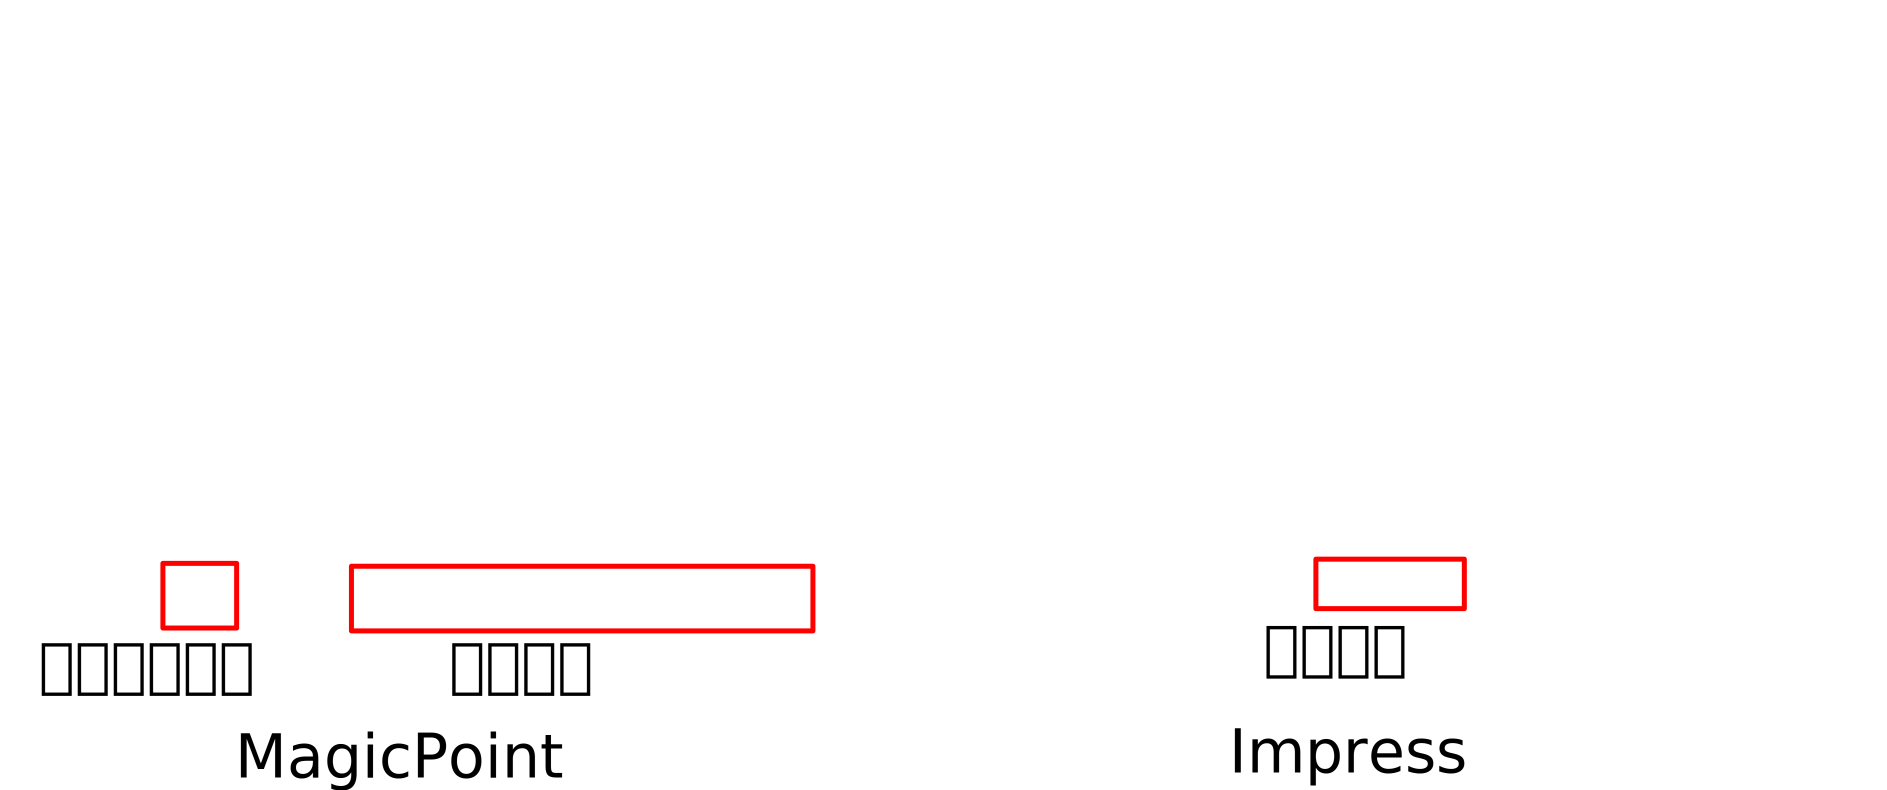
\includegraphics[width=1\hsize]{images/normal-timer-ui.eps}
  \end{center}
  \caption{従来のタイマー機能のUI}
  \label{fig:normal-timer-ui}
\end{figure}

一方、RabbitのUIは発表者だけではなく観客にもわかりやすく表示します。
図\ref{fig:rabbit-timer-ui}のように、スライド下部にうさぎとかめを表示し
ます。それも誰が見ても気づくくらいの大きさで表示します。このようにタイ
マー機能を観客からもわかりやすく表示するUIは既存のプレゼンテーションツー
ルとは一線を画します。

\begin{figure}[ht]
  \begin{center}
    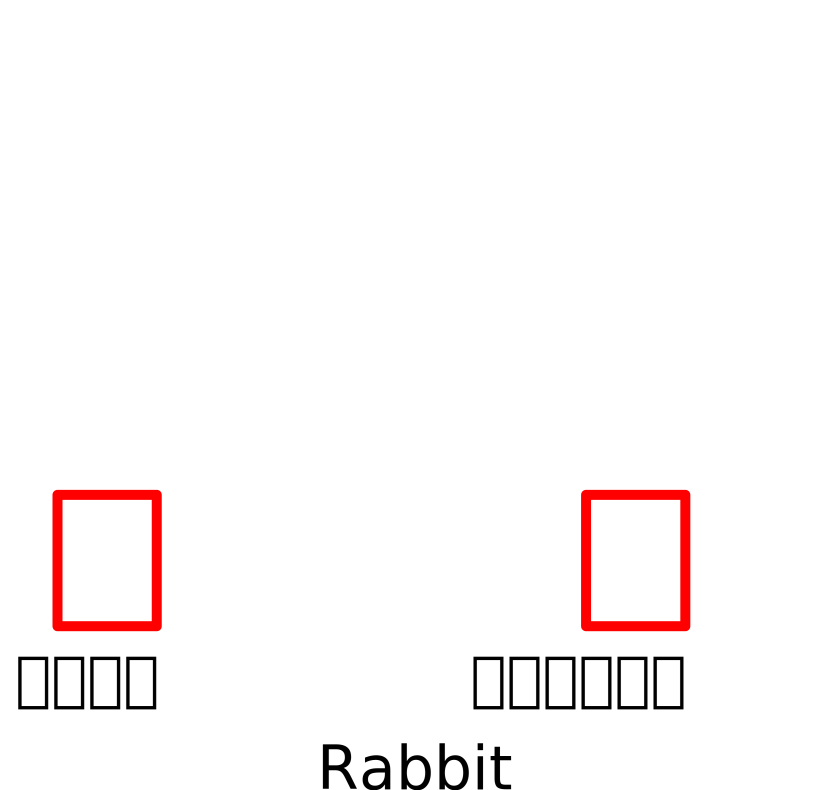
\includegraphics[width=0.5\hsize]{images/rabbit-timer-ui.eps}
  \end{center}
  \caption{Rabbitのタイマー機能のUI}
  \label{fig:rabbit-timer-ui}
\end{figure}

それでは、このUIがどうして時間内に終わるための効果を提供するかを考えて
みましょう。

\subsubsection{みんなにわかる}

このRabbitのUIの特徴は発表者だけではなく、観客にも発表の進み具合がわか
りやすいという点です。発表時間を過ぎれば経過時間を表しているかめが画面
の右側に走りすぎていきます。もちろん、かめなので徐々に画面の右側に進ん
でいきます。そのため、観客が気づかないうちに発表時間を過ぎていたという
ことが起きなくなります。発表時間を過ぎても終わらないと、たとえどれだけ
魅力的な話であっても気まずい空気になってきます\footnote{要出典。}。

発表者は観客の反応がよいとよりすばらしい発表ができますが、逆に反応が悪
いと、準備してきた成果を発揮しづらいものです。発表時間が過ぎても終わら
ない場合、観客の反応が悪くなります。この状態でさらに続けることはとても
つらいので自然と終わらせようとします。

このように、観客からのフィードバックを通じて時間内に終わらせるような発
表に近づきます。もし、発表が長引いてしまった場合でもできるだけ早く終わ
るようになります。

\subsection{インストール方法}

RabbitをDebian GNU/Linuxへインストールする方法を紹介します。インストー
ル方法は以下の2種類あります。

\begin{itemize}
\item aptを使う
\item RubyGemsを使う
\end{itemize}

最新バージョンを使いたい場合やフル機能を使いたい場合はRubyGemsを使う方
法がオススメです。簡単にインストールしたい場合はaptを使う方法がオススメ
です。

\subsubsection{aptでインストール}

まずは、aptを使う方法です。Rabbitのdebパッケージは公式aptリポジトリに含
まれている\footnote{大統一Debian勉強会の実行委員でもある佐々木洋平さん
がパッケージメンテナー。}ので以下のようにすれば簡単にインストールできます。

\begin{commandline}
% sudo apt-get -V -y install rabbit
\end{commandline}

以下のコマンドを実行してスライドが表示されたら正常にインストールできています。

\begin{commandline}
% rabbit https://raw.github.com/shockers/rabbit/master/sample/theme-bench.rab
\end{commandline}

\subsubsection{RubyGemsでインストール}

次にRubyGemsを使う方法です。RabbitはGTK+などたくさんのライブラリを利用
しています。そのため、まず、関連ライブラリをaptでインストールします。

\begin{commandline}
% sudo apt-get -V -y install \
    ruby1.9.1 ruby1.9.1-dev libgtk2.0-dev librsvg2-dev libpoppler-glib-dev \
    libxml2-dev libxslt1-dev
\end{commandline}

関連ライブラリをインストールしたらRubyGemsでRabbitをインストールします。

\begin{commandline}
% sudo gem1.9.1 install rabbit twitter-stream twitter_oauth
\end{commandline}

以下のコマンドを実行してスライドが表示されたら正常にインストールできています。

\begin{commandline}
% PATH="/var/lib/gems/1.9.1/bin:$PATH"
% rabbit https://raw.github.com/shockers/rabbit/master/sample/theme-bench.rab
\end{commandline}

\subsection{スライドの作り方}

RabbitはMagicPointや\TeX{}のようにテキストでスライドを作成します。テキ
ストのフォーマットにはRD\footnote{Ruby Documentの略。}やWiki形
式、Markdownなどいくつもの有名なフォーマットをサポートしています。ここ
では、RDでのスライドの書き方を紹介します。

\subsubsection{RDでのスライドの作り方}

RDでスライドを作る場合、以下のように「\tt{=}」でスライドを区切ります。
「\tt{=}」の行に書いているテキストがそのスライドのタイトルになります。
シンプルですね。

\begin{screen}
\begin{alltt}
# slide.rab

= タイトルスライド

# 持ち時間
: allotted-time
   5m

= 最初のスライド

  * 1枚目のスライドの内容

= 2枚目のスライド

  * 2枚目のスライドの内容
\end{alltt}
\end{screen}

最初のスライドは特別でタイトルスライドになります。ここにはスライド全体
のメタデータを指定することができます。「\tt{allotted-time}」というのは
このプレゼンテーションの持ち時間で、「\tt{5m}」は5分\footnote{5
  Minutes}という意味です。持ち時間を指定するとうさぎとかめタイマーが表
示されるので、持ち時間が決まっているプレゼンテーションのときは指定しま
しょう。

作成したスライドは以下のように実行します。2ページ目以降を表示するとうさ
ぎとかめタイマーが動きだします。

\begin{commandline}
% rabbit slide.rab
\end{commandline}

\subsubsection{PDFで作成したスライドの表示方法}

Rabbitはスライドを表示する機能だけを提供しているため、スライド作成を支
援する機能はありません。Debian GNU/Linuxを使っている人はエディターでテ
キストを編集することに慣れているでしょうが、たまにはImpressなどを使っ
てGUIでグラフィカルにスライドを作成したくなるかもしれません。そのときは
そのようなツールでスライドを作成してください。Rabbitはテキストだけでは
なくPDFファイルも読むこむことができます。Impressなどでスライドを作成
し、PDFで出力すればRabbitで表示することができます。

PDFを表示するときはコマンドラインから持ち時間を指定しま
す。\tt{--allotted-time 5m}と指定すると持ち時間が5分という意味になりま
す。PDFを表示する場合は2ページ目以降からうさぎとかめタイマーが動きだします。

\begin{commandline}
% rabbit --allotted-time 5m slide.pdf
\end{commandline}

\subsection{さいごに}

Debian GNU/Linux上で動作する時間内に終われるプレゼンテーションツー
ルRabbitを紹介しました。Debian GNU/Linuxでプレゼンテーションをする人た
ちの参考になることを期待しています。

\end{document}
